\documentclass[11pt]{article}
\usepackage[utf8]{inputenc}
\usepackage[english]{babel}
\usepackage{pdfpages}
\usepackage{hyperref}
\usepackage{float}
\usepackage{verbatim}
\usepackage{graphicx}
\usepackage{systeme}
\title{Network}
\author{Riccardo Scheda}

\begin{document}

%\maketitle

\section{Random Boolean Networks}

Let's consider a network of $N$ nodes. The state of each node at a time $t$ is given by $\sigma_i(t) \in {0,1}$ with $ i = 1,...,N$.
The $N$ nodes of the network can therefore together assume $2^N$ different states.
The number of incoming links to each node $i$  is denoted by $k_i$ and is drawn
randomly independently from the distribution $P(k_i)$.
The dynamical state of each $\sigma_i(t)$ is updated synchronously by a Boolean function $\Lambda_i$:
$$
\Lambda_i:\{0,1\}^{k_i} \to \{0,1\}
$$ 
An update function specifies
the state of a node in the next time step, given the state
of its $K$ inputs at the present time step. Since each of the
$K$ inputs of a node can be on or off, there are $M = 2^K$ possible input states.
The update function has to specify the new state of a node for each of these input states.
Consequently, there are $2^M$ different update functions.
Fo example let's consider a network with $K=1$, so all the functions $\Lambda_i$ receives the input from one single node. We can see the different possible functions for all the possible networks with $K=1$:

$$
one: \\\Lambda_i(\sigma_j) =  \[ 
\systeme*{1 \;\; $if$ \;\; \sigma_j=0,1 \;\; $if$ \;\;\sigma_j = 1}
\]
$$

$$
zero: \\\Lambda_i(\sigma_j) =  \[ 
\systeme*{0 \;\; $if$ \;\; \sigma_j=0,0 \;\; $if$ \;\;\sigma_j = 1}
\]
$$

$$
copy: \\\Lambda_i(\sigma_j) =  \[ 
\systeme*{0 \;\; $if$ \;\; \sigma_j=0,1 \;\; $if$ \;\;\sigma_j = 1}
\]
$$

$$
invert: \\\Lambda_i(\sigma_j) =  \[ 
\systeme*{1 \;\; $if$ \;\; \sigma_j=0,0 \;\; $if$ \;\;\sigma_j = 1}
\]
$$

Now, in general each element 
receives inputs from exactly $K$ nodes, so we have a dynamical system defined from:

\begin{equation}
\sigma_i(t+1)=\Lambda_i(\sigma_{i_1}(t),\sigma_{i_2}(t), ...,\sigma_{i_K}(t)).
\end{equation}  

So, the randomness of these network appears at two levels: in the connectivity of the network (which node is linked
to which) and the dynamics (which function is attributed to which node).

But, once the links and the functions $\Lambda_i$ are fixed, the evolution of the configurations is deterministic and since we have finite $N$ number of nodes, the evolution becomes periodic. 

\begin{figure}[ht!]
  \center
  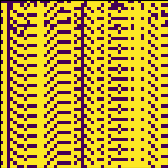
\includegraphics[scale=0.5]{rbn.png}
 \caption{Example of the evolution of random boolean network with $N=50$, $K=1$.}
  \label{fig:net}
\end{figure}

\section{Attractors}
All nodes are updated at the same time
according to the state of their inputs and to their update
function. Starting from some initial state, the network
performs a trajectory in state space and eventually arrives on an \emph{attractor}, where the same sequence of states
is periodically repeated. Since the update rule is deterministic, the same state must always be followed by the
same next state. If we represent the network states by
points in the $2^N$-dimensional state space, each of these
points has exactly one “output”, which is the successor
state. We thus obtain a graph in state space.

 In a network where we have $m$ attractors,
we can define the size of an attractor $\omega_s$ with $s = 1,...,m$ as the number of different states on the attractor. The basin of attraction
of an attractor is the set of all states that eventually
end up on this attractor, including the attractor states
themselves.  So we can define the size of the basin of attraction $\Omega_s$ as the
number of states belonging to it. The graph of states
in state space consists of unconnected components, each
of them being a basin of attraction and containing an
attractor, which is a loop in state space. 


Let us consider an example with a network with $N=4$
and $K = 1$  shown in Figure~\ref{fig:rb2}, which consists of 4
nodes:

\begin{figure}[h]
\centering
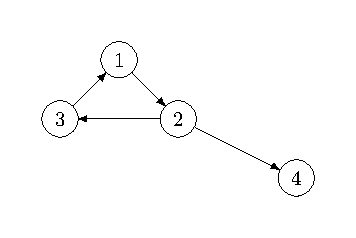
\includegraphics[scale=1]{figurenetworks2.pdf}
\caption{A small network with $N=4$ and $K=1$.}
\label{fig:rb2}
\end{figure}

If we assign to the nodes 1,2,3,4 the functions invert,
invert, copy, copy, an initial state $1111$ evolves in the
following way:

$$
1111 \to 0011 \to 0100 \to 1111
$$

This is an attractor of period 3. If we interpret the bit sequence characterizing the state of the network as a number in binary notation, the sequence of states can also be
written as

$$
15 \to 3 \to 4 \to 15
$$

The entire state space is shown in Figure~\ref{fig:rb3}:
\begin{figure}[h]
\centering
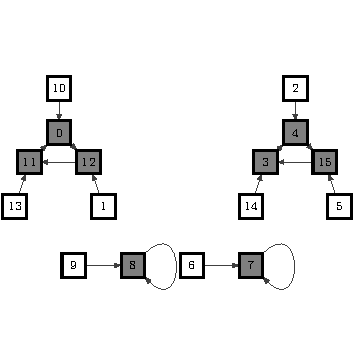
\includegraphics[scale=1]{fg3.pdf}
\caption{The state space of the network shown in Figure~\ref{fig:rb2}, if
the functions copy, copy, invert, invert are assigned to the four
nodes. The numbers in the squares represent states, and arrows indicate the successor of each state. States on attractors
are shaded.}
\label{fig:rb3}
\end{figure}

There are 4 attractors, two of which are fixed points
(i.e., attractors of length $1$). The sizes of the basins of
attraction of the 4 attractors are $\Omega_1=6,\Omega_2= 6,\Omega_3 = 2,\Omega_4 = 2$.

\section{Perturbation}
Since we are talking about gene networks for cell differentiation, we can make some assumptions:

We can consider attractors in the state space as gene regulatory networks of different cells, where different attractors represent cells of different type, and where for example cancer cells lay in one specific attractor.
Now, if we suppose that different cell types lay in different attractors, we can suppose that the jump from an attractor to one other is given by a perturbation in the binary sequence of the genes.
So for example we take the previos network, and consider that we are in the state $12$ of the first attractor:
$$
12 \to 11 \to 0 \to 12
$$

And suddenly we change the state of the third node from $0$ to $1$:
$$
1100 \to 1110
$$

We change the system to have the state $14$ and so we jump into the second attractor:
$$
14 \to 3 \to 4 \to 15 \to 3
$$
\begin{figure}[h]
\centering
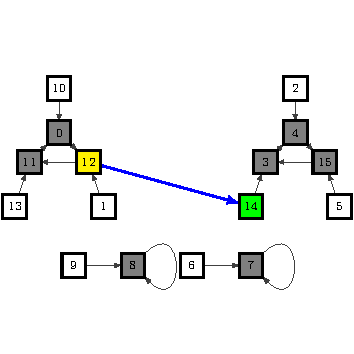
\includegraphics[scale=0.8]{fg4.pdf}
\caption{Jump from one attractor to one other in the state space}
\label{fig:rb4}
\end{figure}


Now, if we consider all the possible perturbations in the binary sequence of the gene, we can get the frequencies of the transitions between the attractors, and what we obtain is an other network, where the nodes are the attractors and the frequencies of transitions can be put in the adjacency matrix of this network.
So in this example we have four attractors, so the network will have the form in Figure~\ref{fig:rb5}.

\begin{figure}[h]
\centering
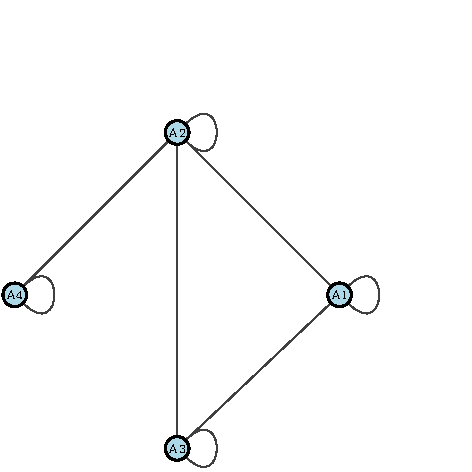
\includegraphics[scale=1]{fg5.pdf}
\caption{Example of the network in the attractor space}
\label{fig:rb5}
\end{figure}

So, having the adjacency matrix formed by the transistion rates from one attractor to one other we can construct a random walk in this network.


\end{document}




First, Kauffman in his work found that there is a phase transition in chaos determined by the parameter $K$, and found that there is a critical $K_c = 2$ for which for $K>K_c = 2$ there system becomes chaotic. For this reason, considering gene regulatory network a stable system, we have to consider networks with $K=1$ input nodes.

